\documentclass[report]{BetterDocument}

\newcommand{\ofc}{Open Food Facts}
\newcommand{\bdd}{base de données}

\title{Buy Or Not}
\subtitle{Doc Technique}
\who{MARTIN Justine}
\date{}
\place{BTS SIO 2 - Jean Rostand Caen}

\begin{document}

	\pageDeGarde

	\tableDesMatieres

	\chapter{Présentation}

	La présente application Android a pour but la gestion des produits en utilisant une \bdd{} semblable à celle d'\ofc{}. En effet, si cette application est satisfaisante, on pourra alors la redévelopper en utilisant cette fois ci la \bdd{} d'\ofc{} tout en s'appuyant sur le code préexistant. Cette documentation a donc pour objectif de présenter le fonctionnement de l'application pour les utilisateurs afin de les accompagner dans la prise en main de celle ci.

	Attention, toutes les fonctionnalités ne sont pas implémentées. L'objectif principal de l'application est respecté cependant des informations comme le pays de provenance, les catégories, etc sont volontairement omises, l'application n'étant actuellement conçue que dans un cadre d'ébauche pour un éventuel développement à plus grande échelle.

	De manière générale, le présent document couvrira uniquement la partie du code de l'application. Celui-ci ne traitera pas des aspects propres à Android comme l'utilisation de Sqlite, les RecyclerView, la bibliothèque AppCompat, la bibliothèque Design, etc. Cependant voici quelques liens afin de vous aiguiller :

	\begin{itemize}
		\item RecyclerView : \url{https://guides.codepath.com/android/Using-the-RecyclerViews}
		\item AppCompat : \url{https://www.captechconsulting.com/blogs/android-material-themes-made-easy-with-appcompat}
		\item Design : \url{https://android-developers.googleblog.com/2015/05/android-design-support-library.html}
	\end{itemize}

	\chapter{Gestion de la \bdd{}}

		Tout le code concernant la \bdd{} est stocké dans le package com.ppe.buyornot.bdd.

		\section{La classe BuyOrNotDatabase}

			Cette classe hérite de la classe SQLiteOpenHelper. La \bdd{} est sauvegardée dans le fichier "BurOrNot.db". La classe utilise le Pattern Singleton. Lors de la création de la \bdd{}, on réeffectue toutes les modifications une à une. Ces modifications sont faites à l'aide de scripts SQL contrairement à ce que l'on a pu voir dans les applications précédentes.

			\begin{figure}[H]
				\centering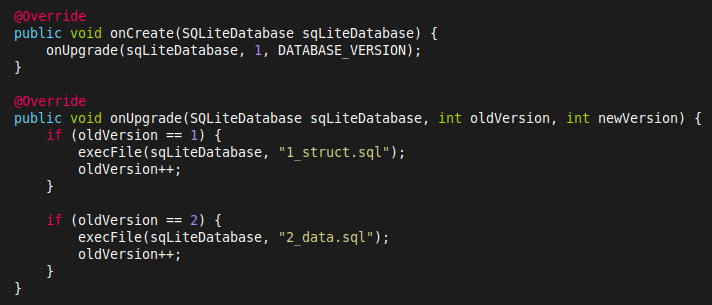
\includegraphics[width=0.75\textwidth, keepaspectratio]{img/bdd/maj_bdd.png}
				\caption{Code de mise à jour de la \bdd{}}
			\end{figure}

			Ainsi à chaque nouvelle version de la \bdd{}, on exécute un script SQL précis en fonction des versions en retard. Pour exécuter ce script, on appelle la fonction "execFile" dont voici le code :

			\begin{figure}[H]
				\centering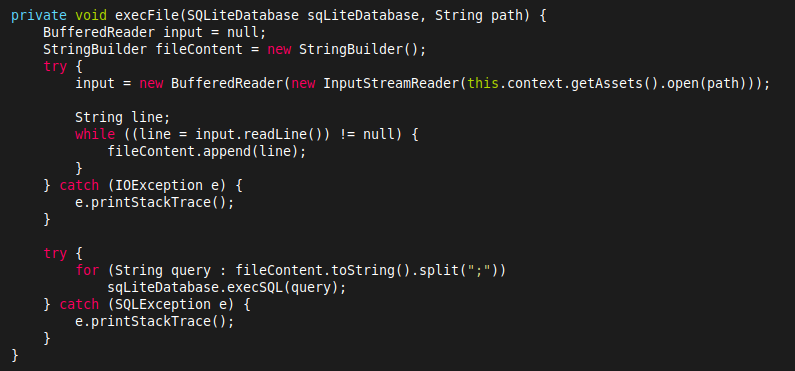
\includegraphics[width=0.75\textwidth, keepaspectratio]{img/bdd/exec_script.png}
				\caption{Code d'exécution d'un script}
			\end{figure}

			Le code n'est rien de plus qu'une simple lecture du fichier SQL fourni en paramètre. La seule subtilité réside dans le fait que pour exécuter le script, on doit exécuter chaque instruction une à une, raison pour laquelle on sépare le contenu du fichier à chaque ";".

		\section{Les scripts de \bdd{}}

			Tous les sripts SQL de la \bdd{} sont contenus dans le dossier suivant : "src/app/src/main/assets". Lorsque l'on veut faire évoluer la \bdd{}, il suffit donc de faire un script SQL et d'exécuter le script correspondant. Il est préférable de respecter la nommenclature visible, à savoir le numéro de version suivi du descriptif du script.

		\section{Les classes modèles}

			Avant d'expliquer comment nous manipulons la \bdd{} afin d'y ajouter ou récupérer des informations, il faut savoir que nous avons dans le package com.ppe.buyornot.bdd.model toutes nos classes métiers. La particularité de celles-ci est qu'elles implémentent l'interface IEntity.

			\begin{figure}[H]
				\centering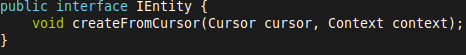
\includegraphics[width=0.75\textwidth, keepaspectratio]{img/bdd/ientity.png}
				\caption{L'interface IEntity}
			\end{figure}

			Cette interface permet d'avoir une base commune pour toutes nos classes métiers. Cependant elle fournit aussi la méthode "createFromCursor" qui prend en paramètre des objets fournis par le SDK d'Android, à savoir un Cursor et un Context. Comme son nom l'indique elle permet de créer une entité depuis un Cursor fournis. Ainsi, appeller cette méthode sur la classe métier "Produit", par exemple, permettra d'obtenir une instance de celle-ci avec toutes ses informations suivant les valeurs du Cursor(ex : le libellé, l'URL, le taux de sucre, etc). Le Context est là pour permettre d'appeler un autre DAO (nous en parlerons dans la partie suivante).

			\begin{figure}[H]
				\centering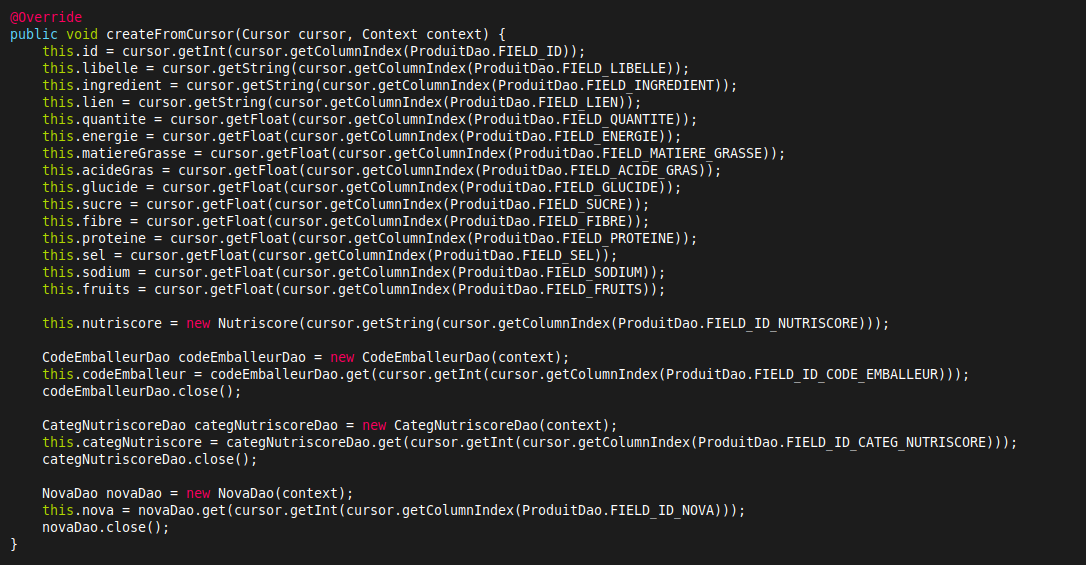
\includegraphics[width=0.75\textwidth, keepaspectratio]{img/bdd/createfromcursor_produit.png}
				\caption{La méthode createFromCursor de la classe Produit}
			\end{figure}

		\section{Pattern DAO}

			Tous les DAO sont disponibles dans le package com.ppe.buyornot.bdd.dao

			Passons maintenant aux explications concernant les DAO. Tous les DAO implémentent l'interface IEntityManager. Cette classe utilise la généricité sur toute classe héritant de l'interface IEntity. On à ainsi plusieurs méthodes qui permettent par exemple de récupérer une entité, d'en ajouter une, d'en supprimer une, etc, le tout uniquement pour la classe T.

			\begin{figure}[H]
				\centering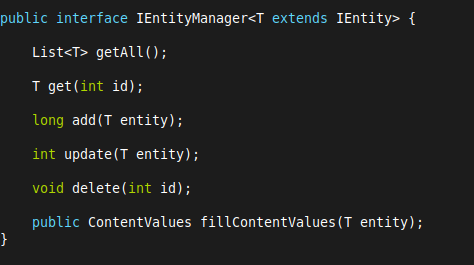
\includegraphics[width=0.75\textwidth, keepaspectratio]{img/bdd/ientitymanager.png}
				\caption{L'interface IEntityManager}
			\end{figure}

			Un avantage de cette méthode est l'utilisation possible du Pattern Strategy pour la création d'une factory (nous en parlerons plus tard).

			Voyons maintenant comment est conçu un DAO :

			\begin{figure}[H]
				\centering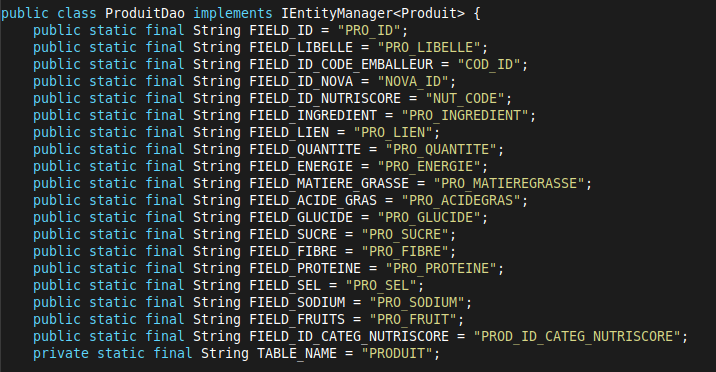
\includegraphics[width=0.75\textwidth, keepaspectratio]{img/bdd/dao_field.png}
				\caption{Base d'un DAO}
			\end{figure}

			Comme on peut le voir, un DAO utilise l'interface IEntityManager et définit des constantes publiques qui permettent de définir les différents champs SQL disponibles sur la table de l'entité.

			\begin{figure}[H]
				\centering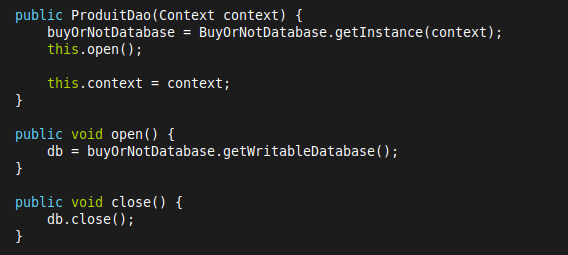
\includegraphics[width=0.75\textwidth, keepaspectratio]{img/bdd/dao_open_close.png}
				\caption{Constructeur et gestion des flux à la \bdd{}}
			\end{figure}

			Ici, on utilise le Context fourni en paramètre afin de récupérer la connexion à la \bdd{}. On définit également 2 méthodes qui permettent de gérer correctement la mémoire en ouvrant ou fermant la connexion active à la \bdd{}.

			\begin{figure}[H]
				\centering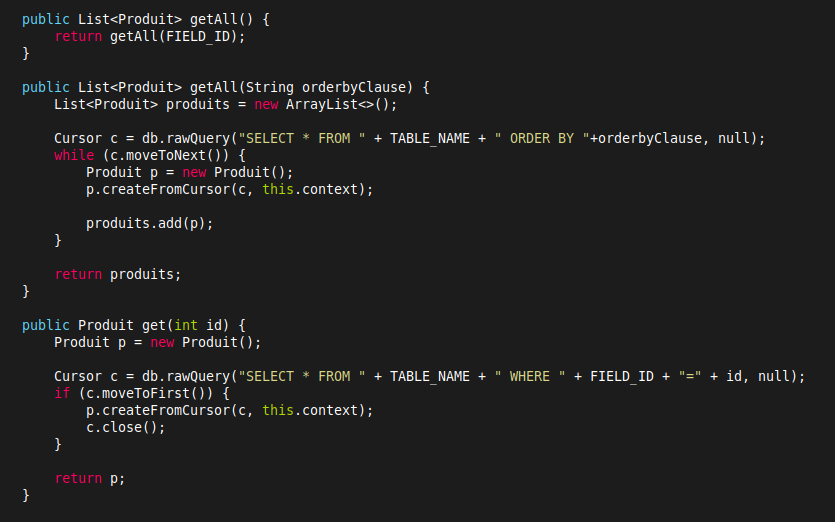
\includegraphics[width=0.75\textwidth, keepaspectratio]{img/bdd/dao_methodes_gets.png}
				\caption{Implémentation des méthodes get(int) et getAll() de IEntityManager}
			\end{figure}

			Le DAO pour les produits est un peu particulier. En effet, la méthode getAll() appelle la méthode getAll(String) afin de trier les éléments dans un certains ordre. L'ordre est défini par la classe String fournie en paramètre. Ainsi, un appel à getAll() retourne les produits triés par ordre d'ajout. Concernant les méthodes get, getAll, on utilise la méthode de l'interface IEntity, à savoir createFromCursor. Ainsi, ici, la création du produit et le changement de ses différents attributs tiennent en 2 lignes seulement et permettent une factorisation du code qui est commun.

			\begin{figure}[H]
				\centering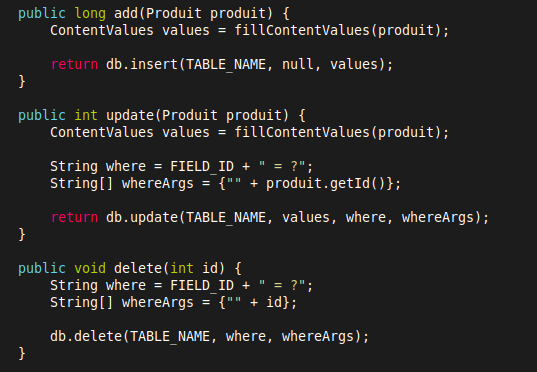
\includegraphics[width=0.75\textwidth, keepaspectratio]{img/bdd/dao_methodes_add_update_delete.png}
				\caption{Implémentation des méthodes add(Produit), update(Produit) et delete(int) de IEntityManager}
			\end{figure}

			Le code de la méthode add et update utilisent donc la méthodes fillContentValues qui permet d'obtenir une instance de ContentValues contenant toutes les informations sur le produit fourni en paramètre. On a ainsi, une fois de plus, une factorisation du code qui simplifie l'ajout et la modification d'un produit. La suppression, elle se contente uniquement de l'id du produit à supprimer.

			\begin{figure}[H]
				\centering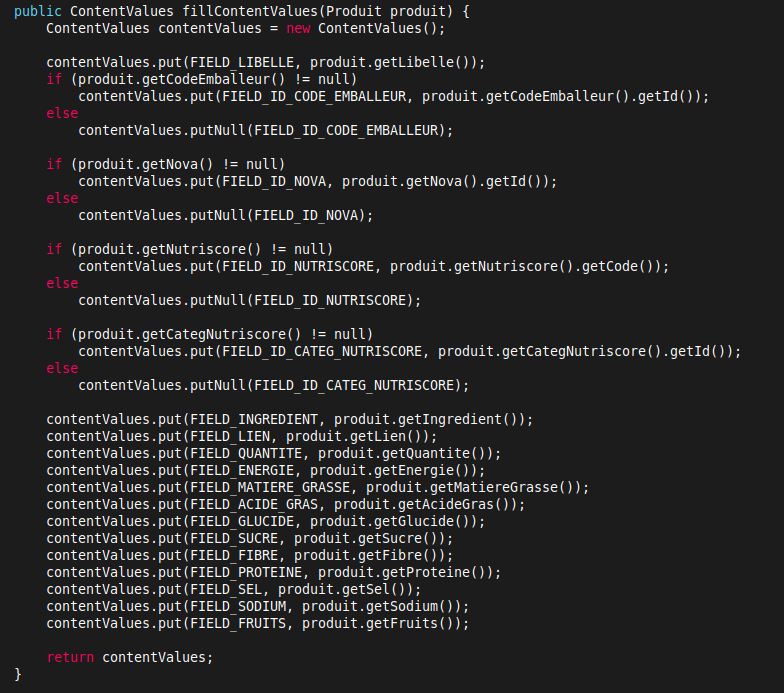
\includegraphics[width=0.75\textwidth, keepaspectratio]{img/bdd/dao_methodes_fillcontentvalues.png}
				\caption{Implémentation de la méthode fillContentValues}
			\end{figure}

			Rien de spécial ici, on instancie un ContentValues que l'on remplit en utilisant le produit en paramètre puis on le retourne.

	\chapter{Les différentes "Activity"}
		\section{MainActivity}

			La classe MainActivity est la 1\iere{} interface que verra l'utilisateur. Celle ci liste les produits par l'intermédiaire d'un RecyclerView en affichant leur nom ainsi que leur nutriscore. Voyons d'abord l'adapter utilisé dans le projet.

			\subsection{Adapter}

				L'adapteur est situé dans le package com.ppe.buyornot.adapter. Pour les produits il s'agit du ProduiRecyclerAdapter. Les adapters pour les RecyclerView faisant partie des bibliothèques support d'Android, leur fonctionnement ne sera pas traité ici. Nous allons uniquement parler de quelques spécificités de la classe.

				\begin{figure}[H]
					\centering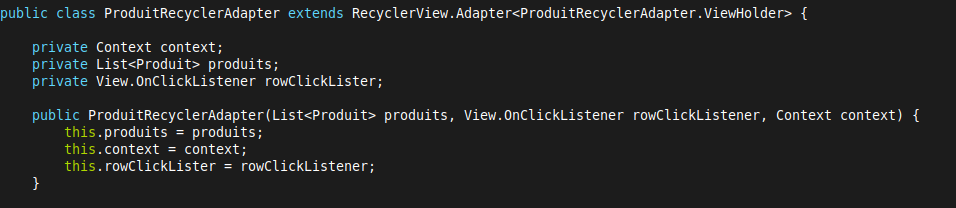
\includegraphics[width=0.75\textwidth, keepaspectratio]{img/adapter/constructor.png}
					\caption{Constructeur de l'adapter}
				\end{figure}

				En effet, pour construire l'adapter on doit fournir la liste des produits à afficher, un OnClickListener ainsi qu'un context. Chacun aura une utilité par la suite.

				\begin{description}
					\item [La liste des produits] Elle permet de lister certains produits. On aurait pu directement faire appel au DAO ici pour récupérer tous les produits, cependant, cela permet de conserver le même code pour lister les produits peut importe que l'on souhaite tout lister ou seulement certains (comme ceux qui ont uniquement un nutriscore en A par exemple).
					\item [L'OnClickListener] Il s'agit du callback pour la sélection d'un item sur la liste. Le fait de le fournir en paramètre ce callback permet de gérer de différentes manières un clic sur un élément de la liste.
					\item[Le Context] Il permet d'obtenir un accès aux Drawables de l'application afin de récupérer celui correspondant au nutriscore du produit que l'on bind.
				\end{description}

			\subsection{Système de tri}

				Le système de tri est rendu possible par la méthode getAll(String) de ProduitDao. Dans le menu "inflaté" on peut alors sélectionner par l'intermédiaire des items la méthode de tri sélectionné.

				\begin{figure}[H]
					\centering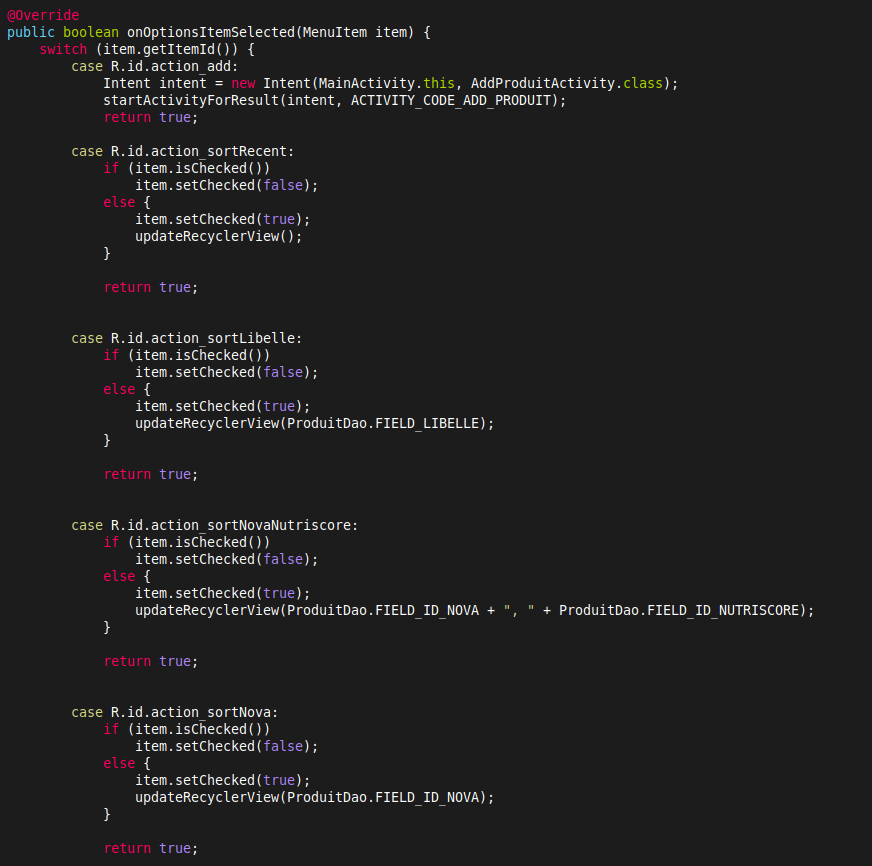
\includegraphics[width=0.75\textwidth, keepaspectratio]{img/activity/MainActivity/sort.png}
					\caption{La gestion des différents tri}
				\end{figure}

				On doit cependant changer manuellement la méthode sélectionnée. Dans le cas où la case ne serait pas cochée, on met alors le RecyclerView à jour en fonction des champs de la \bdd{} fournis par le DAO. Ce tri est fait sous forme de requête SQL.

				\begin{figure}[H]
					\centering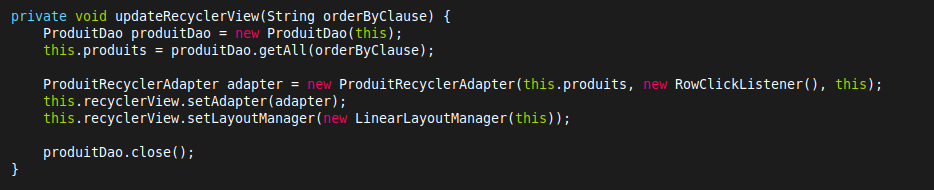
\includegraphics[width=0.75\textwidth, keepaspectratio]{img/activity/MainActivity/update_recyclerview.png}
					\caption{Mise à jour de la RecyclerView}
				\end{figure}

				Rien de spécial dans ce code ci. On utilise la classe ProduitDao afin de récupérer tous les produits triés dans l'ordre demandé. On instancie ensuite l'adapter pour le RecyclerView que l'on utilise directement.

			\subsection{Interaction avec les autres Activity}

				Les activity pour mettre à jour un produit ou pour en ajouter un, retourne un code de résultat. De ce fait il est important de les démarrer en utilisant startActivityForResult(). Ce code de retour permet de savoir si la manipulation du produit a été validée. Si tel est le cas, on doit alors mettre à jour la RecyclerView.

				\begin{figure}[H]
					\centering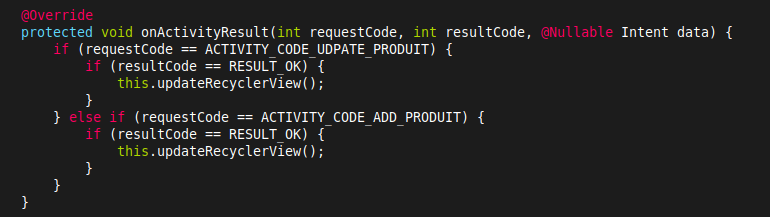
\includegraphics[width=0.75\textwidth, keepaspectratio]{img/activity/MainActivity/onactivityresult.png}
					\caption{Code du OnActivityResult}
				\end{figure}

		\section{AbstractProduitActivity}

			Cette classe fournit une base pour le layout "activity\_produit". Elle permet de récupérer toutes les vues grace à la méthode "findViews()".

			\begin{figure}[H]
				\centering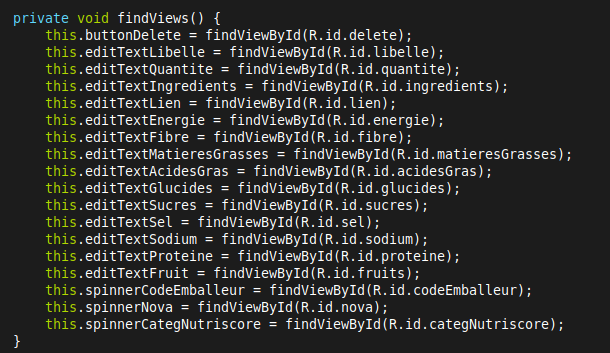
\includegraphics[width=0.75\textwidth, keepaspectratio]{img/activity/AbstractProduitActivity/findviews.png}
				\caption{Code de la méthode findViews()}
			\end{figure}

			On a aussi l'initialisation de tous les spinner de fait. Chaque spinner possède sa propre méthode pour l'initialiser.

			\begin{figure}[H]
				\centering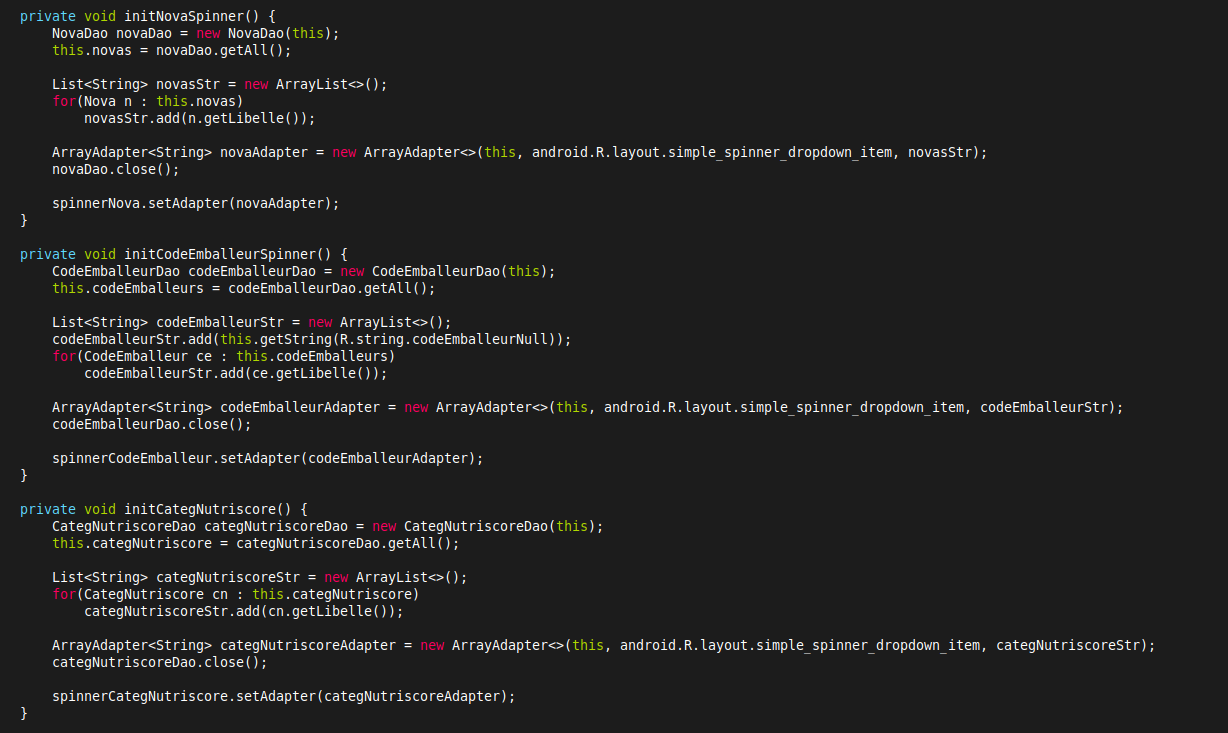
\includegraphics[width=0.75\textwidth, keepaspectratio]{img/activity/AbstractProduitActivity/init_spinners.png}
				\caption{Code d'initialisation des spinner}
			\end{figure}

			De ce fait, les champs étant commun à l'ajout et la modification d'un produit, la classe fournit la méthode getProduit() qui permet de récupérer le produit en fonction de ce ui est actuellement saisie dans les champs. La fonction retournee "null" si un des champs n'est pas remplis, signifiant ainsi une erreur. En effet, il s'agit d'une sécurité visant à vérifier que l'on possède bien les informations du produit. Si l'on ne peut pas renseigner toutes les informations, c'est surement que l'on n'a pas le produit sous les yeux.

			\begin{figure}[H]
				\centering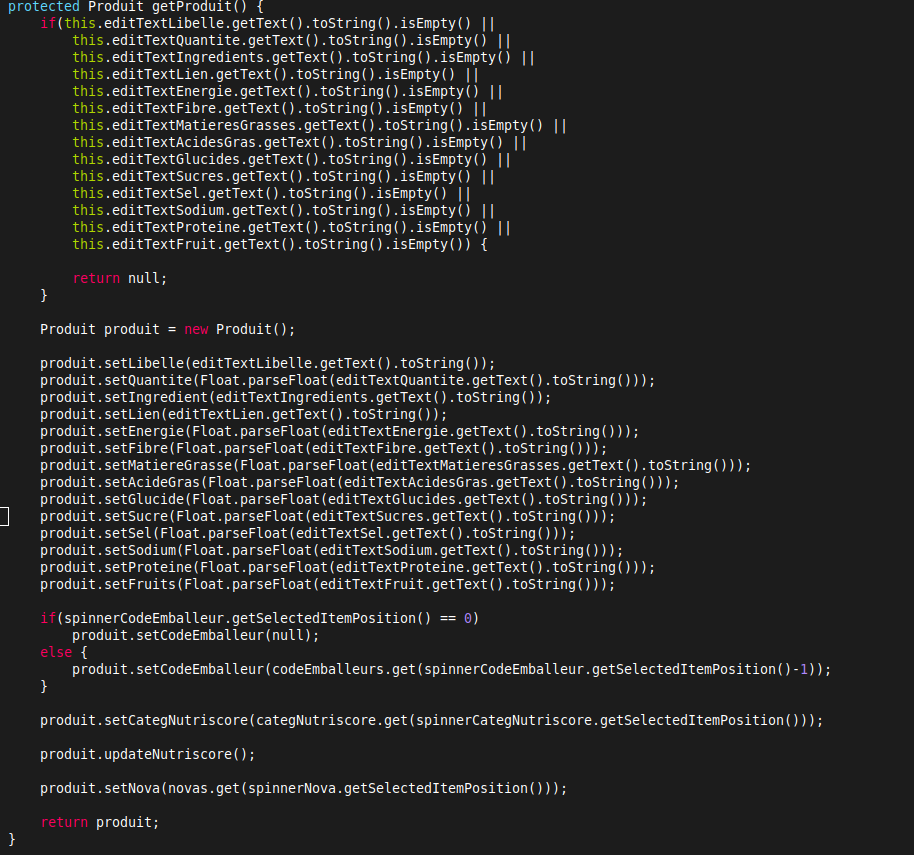
\includegraphics[width=0.75\textwidth, keepaspectratio]{img/activity/AbstractProduitActivity/getProduit.png}
				\caption{Création d'un produit depuis les champs}
			\end{figure}

			En plus de l'interface principale, le menu en haut à droite est le même sur les 2 écrans. De ce fait ce code fournit une méthode abstraite saveProduit() qui permet de définir le comportement à adopter lors d'un clic sur ce bouton.

			\begin{figure}[H]
				\centering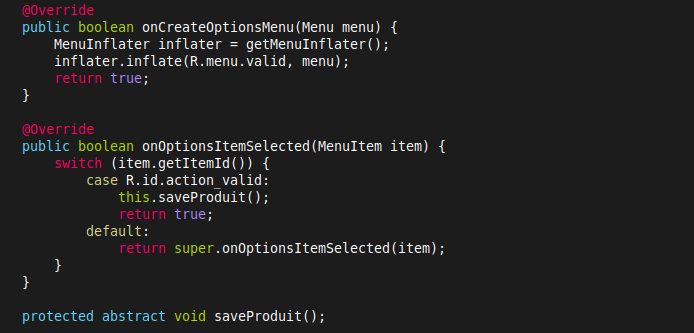
\includegraphics[width=0.75\textwidth, keepaspectratio]{img/activity/AbstractProduitActivity/menu.png}
				\caption{Code d'initialisation des spinner}
			\end{figure}

		\section{AddProduitActivity}

			Cette classe hérite donc de AbstractProduitActivity. La seule spécificité du code est le fait de masquer le bouton pour supprimer. De plus, on implémente la fonction saveProduit() qui se charge uniquement d'afficher le message d'erreur si un des champs est vide ou alors, d'ajouter le produit si tous les champs sont remplis.

			\begin{figure}[H]
				\centering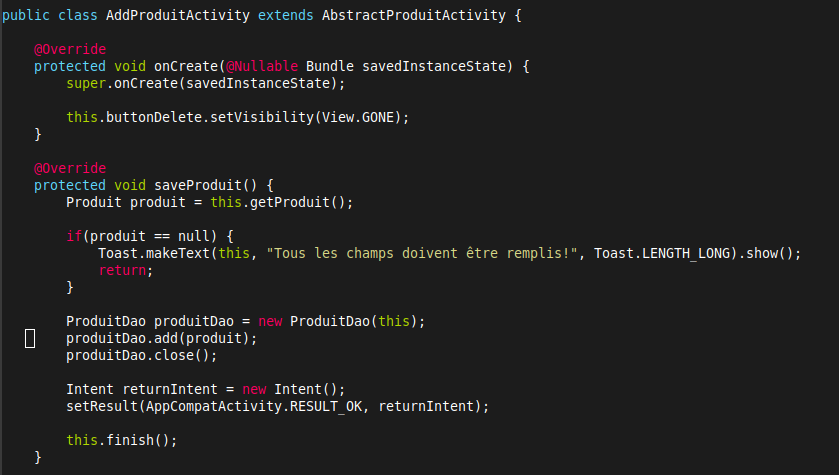
\includegraphics[width=0.75\textwidth, keepaspectratio]{img/activity/AddProduitActivity/code.png}
				\caption{Code de la classe AddProduitActivity}
			\end{figure}

		\section{UpdateProduitActivity}

			Cette classe hérite donc aussi de AbstractProduitActivity. L'id du produit passé en paramètre est récupéré afin de sélectionner le produit correspondant dans la \bdd{}. On exécute alors la méthode updateUi(Produit).

			\begin{figure}[H]
				\centering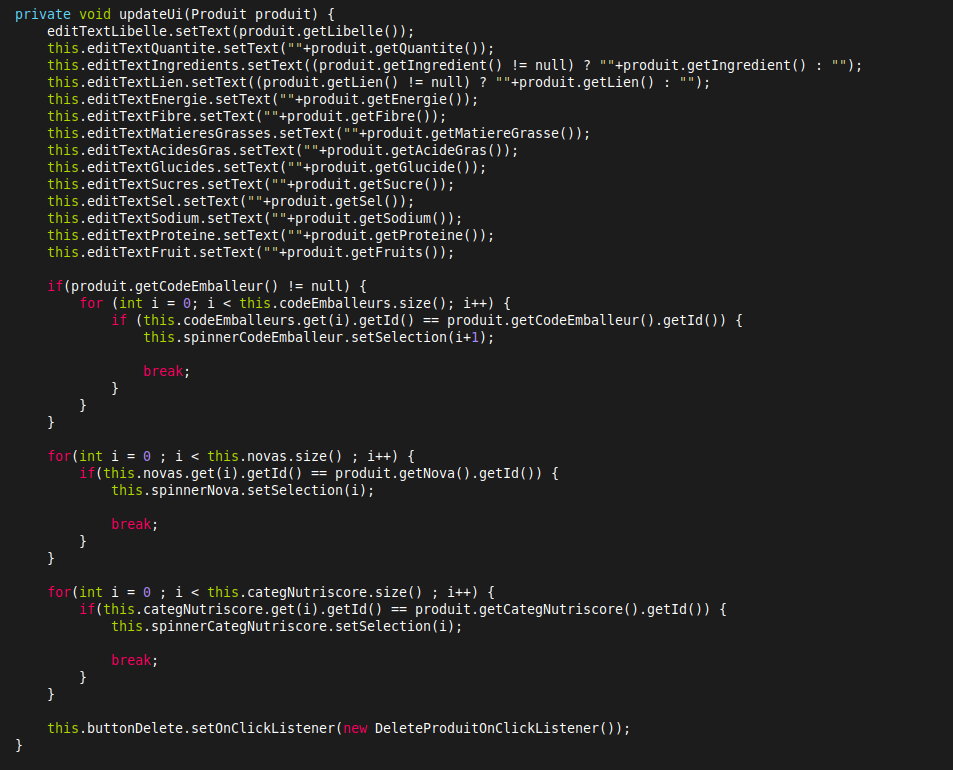
\includegraphics[width=0.75\textwidth, keepaspectratio]{img/activity/UpdateProduitActivity/updateUi.png}
				\caption{Code de la méthode updateUi(Produit)}
			\end{figure}

			De même, le code de saveProduit(Produit) se chargera d'afficher également le message d'erreur ou de mettre à jour le produit correspondant dans la \bdd{}.

			\begin{figure}[H]
				\centering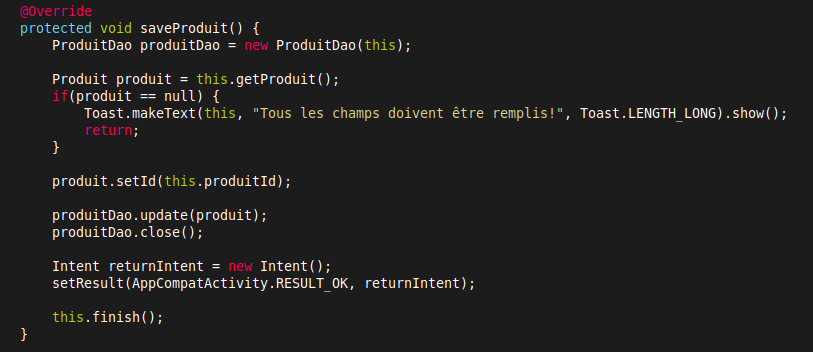
\includegraphics[width=0.75\textwidth, keepaspectratio]{img/activity/UpdateProduitActivity/save.png}
				\caption{Code de la méthode updateUi(Produit)}
			\end{figure}

			Enfin, un OnClickListener existe afin de supprimer le produit en cours de consultation lorsque l'on clique sur le bouton en bas de l'écran.

			\begin{figure}[H]
				\centering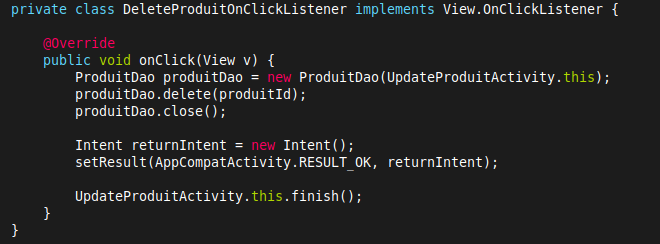
\includegraphics[width=0.75\textwidth, keepaspectratio]{img/activity/UpdateProduitActivity/delete.png}
				\caption{Code de la méthode updateUi(Produit)}
			\end{figure}

	\chapter{Le calcul du Nutriscore}

		Le calcul du nutriscore est fait par la classe NutriscoreCalculator, qui est dans le package com.ppe.buyornot.util. Elle fournit une méthode static getNutriscore(Produit). Cette méthode est l'application du Document 4 du cahier des charges.

		\begin{figure}[H]
			\centering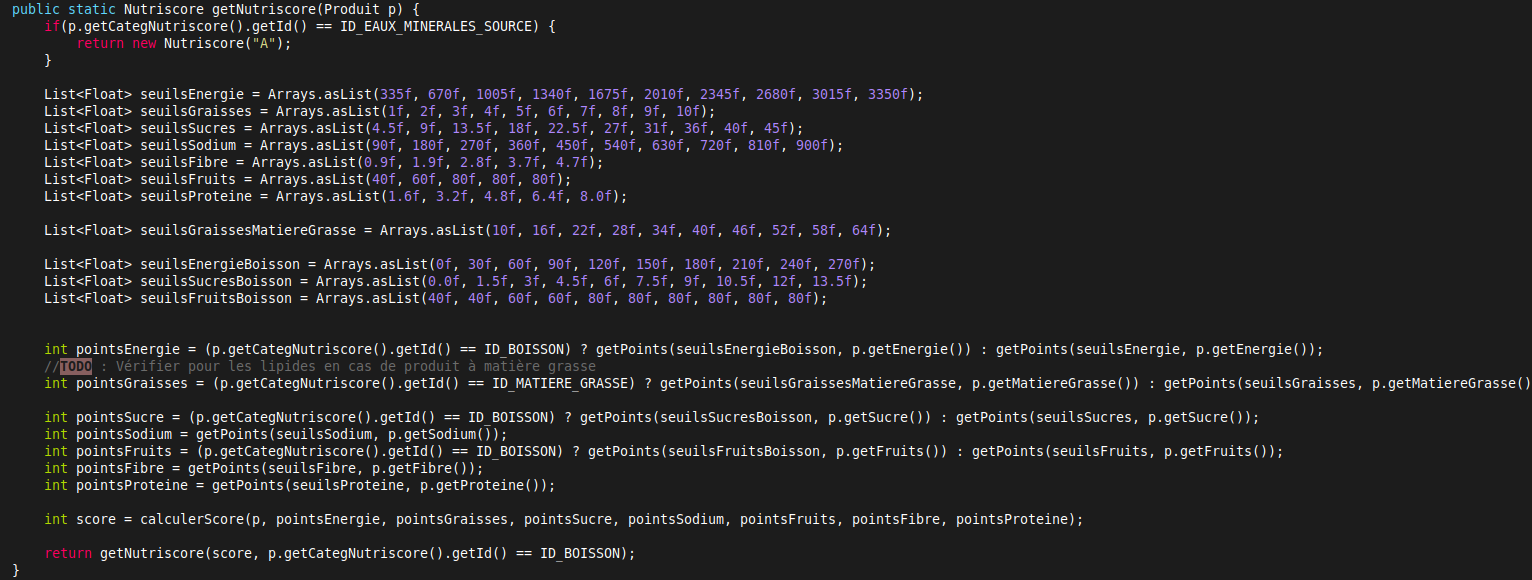
\includegraphics[width=0.75\textwidth, keepaspectratio]{img/util/getNutriscore.png}
			\caption{Code de la méthode getNutriscore(Produit)}
		\end{figure}

		On initialise la liste des seuils pour le calcul des scores. On récupère alors le score pour un élément en récupérant sa "position" dans le tableau à l'aide de la méthode getPoints(List, float).

		\begin{figure}[H]
			\centering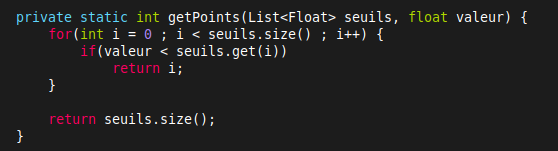
\includegraphics[width=0.75\textwidth, keepaspectratio]{img/util/getPoints.png}
			\caption{Code de la méthode getPoints(List, float)}
		\end{figure}

		On remarque l'utilisation de lignes telles que "p.getCategNutriscore().getId() == CONSTANTE". Cet id peut prendre plusieurs valeurs qui sont répertoriées sous forme de constantes dans la classe. Elles permettent de gérer les adaptations du nutriscore au système français. Ainsi, par exemple, on utilise une expression ternaire pour récupérer le nombre de points en énergie. Cela permet de gérer le cas où le produit est une boisson énergétique.

		Une fois tous les points récupérés, il faut maintenant récupérer le score total en utilisant la méthode calculerScore. Cette méthode permet d'obtenir le score final d'un produit.

		\begin{figure}[H]
			\centering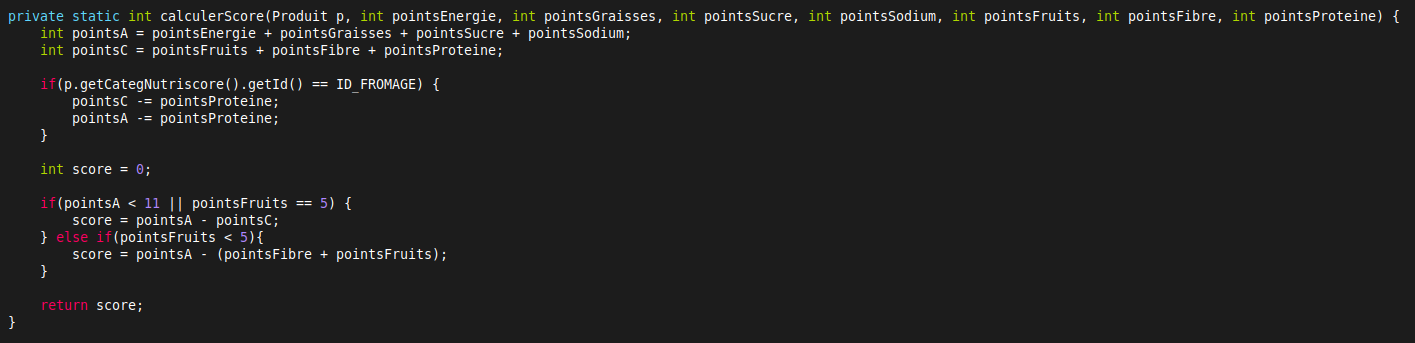
\includegraphics[width=0.75\textwidth, keepaspectratio]{img/util/calculerScore.png}
			\caption{Code de la méthode calculerScore}
		\end{figure}

		Une fois ce score obtenu, getNutriscore(Produit) doit maintenant revoyer le nutriscore associé en utilisant la méthode getNutriscore(int, boolean) (la boolean indiquant s'il s'agit d'une boisson ou non).

		\begin{figure}[H]
			\centering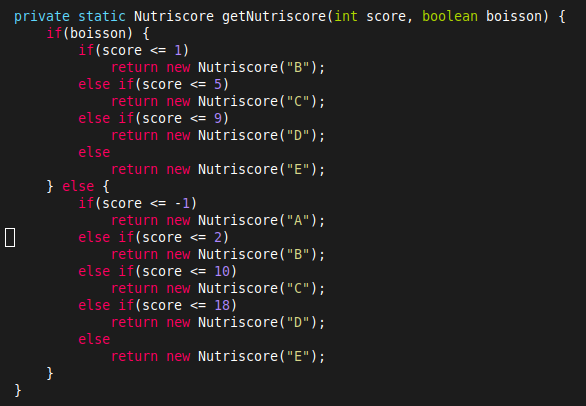
\includegraphics[width=0.75\textwidth, keepaspectratio]{img/util/getNutriscore2.png}
			\caption{Code de la méthode getNutriscore(List, float)}
		\end{figure}

	\chapter{Amélioration importantes}

		\section{Pattern Factory}

			Comme mentionné auparavant, actuellement les fonctions "createFromCursor" fournissent en paramètre une instance de "Context". Cette méthode est relativement contraignante. Dans un développement futur, il faudrait utiliser le pattern Factory afin d'éviter ce genre de contrainte. En effet, il suffit de créer un setter permettant de changer l'instance du Context. Cette méthode serait appelée une seule fois au lancement de l'activité. Par la suite, en utilisant la méthode static "getDao" de la Factory, on pourra alors récupérer le DAO demandé, qui sera créé en utilisant le Context fourni en paramètre plus tôt dans l'activité. On permet donc d'éviter le passage du Context de méthode en méthode et l'on permet aussi une uniformisation et une abstraction de la création et de la gestion des DAO. La factory pourrait ainsi également gérer les méthodes "open" et "close" des DAO, ce qui permettrait une meilleure gestion de la mémoire.

		\section{Implémentation des DAO manquants}

			L'application n'étant là que dans un but de test, tous les DAO ne sont pas implémentés. Il faudra donc tous les créer afin de pouvoir gérer l'ensemble des informations d'un produit.

		\section{Shared Preference}

			Le système de tri se remet à zéro à chaque lancement de l'application. Une amélioration simple et rapide serait de permettre de sauvegarder ce choix dans les SharedPreference d'Android. Cela éviterait de fruster l'utilisateur qui doit actuellement resélectionner à chaque fois son choix pour le tri.

		\section{Utilisation des Fragment}

			Il pourrait également être interessant d'utiliser des Fragment afin de permettre, notamment, une meilleure gestion des interfaces sur mobile et tablette. Voici un article présentant de manière brève leur utilisation \url{https://mathias-seguy.developpez.com/tutoriels/android/comprendre-fragments/}.


	\chapter{Ressources}

		\noindent Développeuse du projet : MARTIN Justine\\
		Adresse mail : \href{mailto:justine.martin.dev@gmail.com}{justine.martin.dev@gmail.com}\\
		Github du projet : \url{https://github.com/justine-martin-study/BuyOrNot}\\
		Trello : \url{https://trello.com/b/HCXYRgZp/buy-or-not}

\end{document}
